El factor de estructura de un sistema se define como la \emph{amplitud de scattering}~\cite{egami_underneath_2003}

\begin{equation}
  \Psi(\mathbf{Q}) = \frac{1}{\langle b\rangle} \sum_i b_i
  \text{e}^{i\mathbf{Q}\cdot\mathbf{R}_i}
  \label{eq:scat_amp}
\end{equation}

con $\mathbf{Q}$ el vector de difracción o transferencia de momento.
$\mathbf{R}_i$ es la posición de la partícula $i$, y $\langle b\rangle$ es el promeedio de la amplitud de scattering de cada partícula en el vacío $b_i$.
A partir de este momento, vamos a considerar que todas las partículas son de la misma especie, $b_i = b$.

A partir de $\Psi(\mathbf{Q})$ definimos $S(\mathbf{Q})$ como

\begin{equation*}
  S(\mathbf{Q}) = \frac{1}{N} |\Psi(\mathbf{Q})|^2
\end{equation*}

La conclusión \emph{inmediata} de esta expresión es que el factor de estructura debe ser positivo siempre para todo valor de $\mathbf{Q}$.
Podemos expandir la amplitud de scattering y utilizar $|z|^2 = z\cdot z^*$  y, si todos los átomos son del mismo tipo,


\begin{align*}
  S(\mathbf{Q}) &= \frac{1}{N} \left( \sum_i \text{e}^{i\mathbf{Q}\cdot\mathbf{R}_i} \right)
  \left( \sum_j \text{e}^{-i\mathbf{Q}\cdot\mathbf{R}_j} \right)\\
  &= \frac{1}{N} \sum_{i, j} \text{e}^{i\mathbf{Q}\cdot(\mathbf{R}_i-\mathbf{R}_j)}\\
  &= \frac{1}{N} \left[N + \sum_{i < j}
    \left(\text{e}^{i\mathbf{Q}\cdot(\mathbf{R}_i-\mathbf{R}_j)} +
      \text{e}^{i\mathbf{Q}\cdot(\mathbf{R}_i-\mathbf{R}_j)}\right)\right]\\
  &= 1 + \frac{2}{N}\sum_{i < j}\cos{\mathbf{Q}\cdot\mathbf{R}_{ij}}
\end{align*}

Usualmente estamos interesados en el conocido como \emph{promedio de polvo} del factor de estructura: es decir, el factor de estructura promediado para todas las posibles orientaciones del vector de difracción (ya que en un polvo tenemos muchas estrucutras orientadas al azar).
Calculamos entonces

\begin{equation*}
  S(q) = \frac{1}{4\pi}\int\text{d}\phi\text{d}(\cos\theta) S(\mathbf{Q})
\end{equation*}

Esta integral puede ser calculada fácilmente si colocamos el eje $z$ en la dirección de $\mathbf{Q}$ e integramos rotando las distancias $\mathbf{R}_{ij}$

\begin{align*}
  S(q) &= \frac{1}{4\pi}\int\text{d}\phi\text{d}(\cos\theta)
  \left[1 + 2\sum_{i < j}\cos\left(q\,r_{ij}\,\cos\theta\right)\right]\\
  &= 1 + \frac{1}{2N}\int\text{d}(\cos\theta)
  2\sum_{i < j}\cos\left(q\,r_{ij}\,\cos\theta\right)\\
  &= 1 + \frac{1}{2N} 2 \sum_{i < j} \left.\frac{\sin(q\,r_{ij}u)}{q\,r_{ij}}\right|_{u=-1}^{u=1}\\
  &= 1 + \frac{2}{N} \sum_{i < j}\frac{\sin(q\,r_{ij})}{q\,r_{ij}}
\end{align*}

Esta es la famosa fórmula de Debye y, como es el promedio de una cantidad que es siempre positiva, debe ser siempre positiva.

Uno de los problemas más usuales cuando modelamos y estudiamos sitemas en simulaciones computacionales es que no tenemos \emph{realmente} sistemas infinitos.
Usamos, para emular el comportamiento de sistemas infinitos, condiciones periódicas de contorno (CPC).
Con las condiciones periódicas de contorno utilizamos la convención de la mínima imagen: de todas las posiciones posibles a través de los contornos para las partículas $i$ and $j$, escogemos el par más cercano.
Utilizando este método para un caso de prueba muy simple (una red cúbica simple tridimensional con 4x4x4=64 partículas) calculamos el factor de estructura que se puede ver en la figura~\ref{fig:ssf_comp}.

\begin{figure}
  \centering
  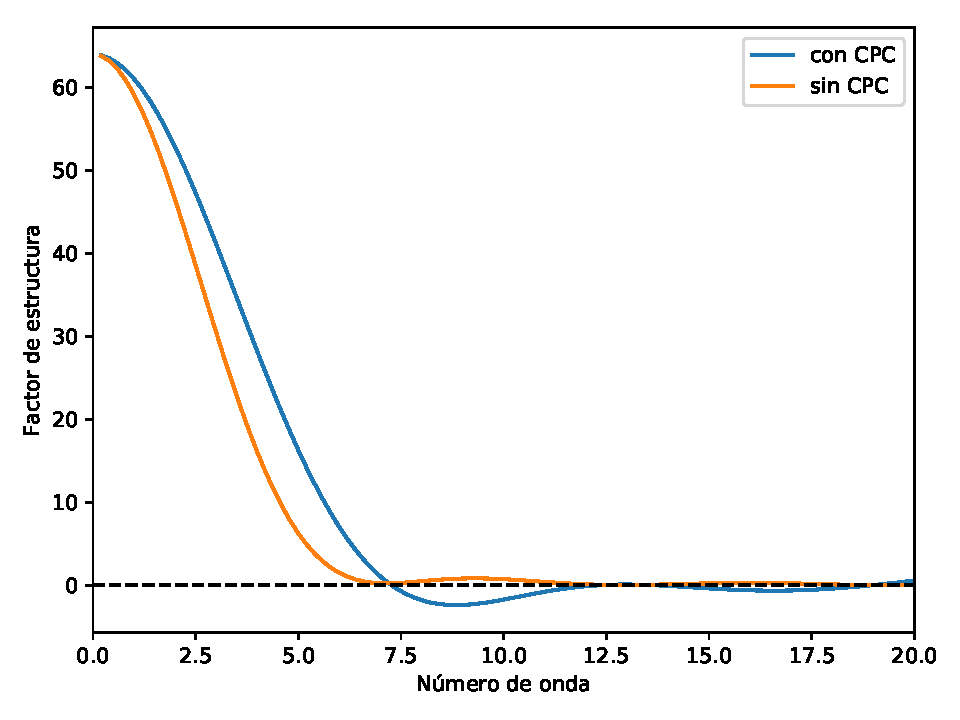
\includegraphics[width=0.4\columnwidth]{nuevas_pastas/ssf_comp.pdf}
  \caption{Comparación del factor de estructura con y sin CPC.
    Es evidente que el factor de estructura calculado con CPC muestra valores negativos, que no deberían existir desde la misma definición del factor de estructura.}
  \label{fig:ssf_comp}
\end{figure}

Podemos ver que el factor de estructura calculado con CPC genera valures negativos, a pesar de que estos valores deberían estar prohibidos.
La razón por la que esto sucede es la convención de mínima imagen: la distancia entre los pares ahroa no es siempre $r_{ij} = r_j - r_i$, sino que depende de si utilizamos las particulas originales o sus imágenes.
En consecuencia, este ``nuevo'' factor de estrucutra no es el producto de dos complejos conjugados\footnote{Más aún, ahora la parte imaginaria de $S(Q)$ ya no es}.
Para explorar el efecto que tiene la convención de la mínima imagen tiene en el factor de estructura, mostramos una comparación del factor de estructura con y sin condiciones de contorno (es decir, con los 64 átomos en el vacío) en la figura~\ref{fig:ssf_comp}.

Esto muestra que el factor de estructura, cuando utilizamos su definición, \emph{sin la convención de la mínima imagen}, es (como era de esperar) siempre positivo.

La pregunta persiste: ¿cómo podemos simular un medio infinito cuando calculamos factores de estructura?
La primera respuesta es que no es obvio que esto pueda ayudar en un medio realmente infinito, ya que las imágenes periódicas de la celda estarían alineadas en un crista lq ue puede interferir con la estructura dentro de la celda (la que queremos estudiar).
Sin embargo, unas pocas réplicas podrían ser suficientes para borrar considerablemente los efectos de tamaño finito.
Una posibilidad es replicar explícitamente la caja, creando las partículas en las celdas vecinas, multiplicando las originales,
Esto, sin embargo, implica un calculo mucho más difícil, ya que la suma para calcular la función de distribución de pares es sobre $N^2$ particles, y replciarla sólo una celda a la derecha y a la izquierda en cada dirección implicaría un tiempo computacional de  $(3^3\cdot N)^2 \approx 700\cdot N^2$.
En general, la complejidad $\mathcal{O}(N^2)$ hace que el cálculo del factor de estructura sea muy costoso para sistemas grandes.

Hay una alternativa para agregar las condiciones de contorno.
Comenzamos con la definición de la \emph{amplitud de scattering} como en~\ref{eq:scat_amp}, pero escribiendo explícitamente las imágenes que queremos considerar:
\begin{equation}
  \Psi(\mathbf{Q}) = \sum_i \sum_j
  \text{e}^{i\mathbf{Q}\cdot(\mathbf{R}_i+\mathbf{\Delta L}_j})
\end{equation}
donde $\mathbf{\Delta L}_j$ es la distancia entre una partícula y su réplica
$j$-ésima. Como las sumas son independientes, podemos escribir:
\begin{equation}
  \Psi(\mathbf{Q}) = \left(\sum_i
    \text{e}^{i\mathbf{Q}\cdot\mathbf{R}_i}\right)
  \left(\sum_j\text{e}^{i\mathbf{Q}\cdot\mathbf{\Delta L}_j}\right)
\end{equation}

Multiplicando por el conjugado, obtenemos el factor de estructura
\begin{align}
  S(\mathbf{Q}) &= \left|\sum_i
    \text{e}^{i\mathbf{Q}\cdot\mathbf{R}_i}\right|^2 \left|\sum_j
    \text{e}^{i\mathbf{Q}\cdot\mathbf{\Delta L}_j}\right|^2\\
  &= S_{\text{cell}}(\mathbf{Q})\,S_{\text{PBC}}(\mathbf{Q})
\end{align}

La ventaja de este cálculo es que es lineal en la suma del número de partículas y el número de répicas que consideremos, $\mathcal{O}(N+M)$, mucho menor que el previo $\mathcal{O}(N^2M^2)$.
En consecuencia, si queremos concentranos en una región de $\mathbf{Q}$, este nuevo enfoque será útil\footnote{Consideremos que con este método necesitamos $\mathcal{O}(N+M)$ cálulos para cada $\mathbf{Q}$, así que no podemos utilizarlo para barrer todo el espectro de $\mathbf{Q}$}.
Quedamos con sólo un datalle, respecto del \emph{powder average}.
No es trivial cómo calcular esta integral, ya que necesitamos darle pesos adecuados a cada ángulo.
En este trabajo utilizamos la cuadratura de Lebedev~\cite{lebedev_values_1975}, aunque otros métodos (como Muestreo por Importancia de Montecarlo) pueden ser útiles en esta situación.